\documentclass[a4paper, 12pt]{article}
% math symbols
\usepackage{amssymb}
\usepackage{amsmath}
\usepackage{mathrsfs}
\usepackage{physsummer}


\usepackage{enumitem}
\usepackage[margin = 2cm]{geometry}

\tolerance = 1000
\emergencystretch = 0.74cm



\pagestyle{empty}
\parindent = 0mm

\begin{document}

\begin{center}
  \Large{\textbf{11 класс.}\\
  \textit{19 ноября 2014.}}
\end{center}


\begin{center}
  \Large \textbf{ Движение в магнитном поле.}
\end{center}

\large

\task{ Длинный цилиндрический соленоид диаметра $d$ создаёт внутри
  себя однородное магнитное поле с индукцией $B_0$. На расстоянии
  $L=5d$ от оси соленоида находится массивная заряженная частица массы
  $M$ с зарядом $Q$. Ток через соленоид отключают, при этом поле
  быстро уменьшается до нуля. С какой скоростью будет двигаться
  частица после отключения поля? }
% Зильберман, ШФО, стр. 148

\task{ Маленький цилиндрический магнит создаёт на своей оси (она
  вертикальна) магнитное поле, направленное вдоль этой оси. На большом
  расстоянии от магнита в интересующей нас области пространства можно
  считать, что поле убывает вдоль этой оси по закону $B = B_0 ( 1-
  ax)$, где $x$~---~расстояние до магнита. Маленькое массивное
  проводящее кольцо падает под действием поля тяжести и магнитного
  поля с установившейся скоростью. Центр кольца всё время находится на
  оси магнита, масса кольца $M$, диаметр кольца $d$, сопротивление
  материала равно $R$. Найдите скорость движения кольца. }
% Зильберман, ШФО, стр. 150

\task{ Тонкий проводящий диск толщиной $d$ и площадью $S$ падает в
  вертикальном положении в горизонтальном магнитном поле индукцией $B$,
  линии которой параллельны плоскости проводника. Найдите ускорение, с
  которым падает диск, если его масса $m$. }

% Hint: от одной поверхности к другой протекает горизонтальный ток, на
% который действует сила Ампера

\taskpic{ Положительно заряженная частица движется в однородных и
  взаимно перпендикулярных электрическом и магнитном полях. В
  некоторый момент времени её скорость равна $\vec{v}_0$ ($\vec{v}_0
  \perp \vec{E}$ и $\vec{v}_0 \perp \vec{B}$). Чему будет равна
  величина скорости частицы в те моменты времени, когда вектор её
  скорости будет составлять $180^{\circ}$ с вектором $\vec{v}_0$, при
  условии что $E = v_0 B$? Поле тяжести не учитывать.}
{
  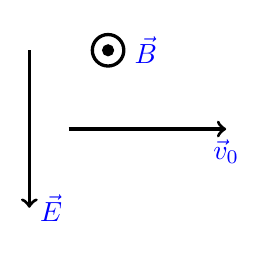
\begin{tikzpicture}
    \draw[very thick,->] (0,2) -- (0,0) node[right,blue] {$\vec{E}$};
    \draw[very thick,->] (0.5,1) -- (2.5,1) node[below,blue]
    {$\vec{v}_0$};
    \draw[very thick] (1,2) circle (0.2cm) node[right=0.2cm,blue] {$\vec{B}$};
    \draw[fill=black] (1,2) circle (0.07cm); 
  \end{tikzpicture}
}
% Квант, практикум абитуриента, 1999-3

\task{ В однородном магнитном поле вращается по круговой орбите
  электрон. Индукцию поля медленно (за время, во много раз превышающее
  период обращения) увеличивают в три раза. Во сколько раз изменится
  радиус орбиты электрона?  }
% Квант, Ф1265, 1991-04

\end{document}


%%% Local Variables: 
%%% mode: latex
%%% TeX-engine:xetex
%%% TeX-PDF-mode: t
%%% End:
